% Short talk: the phase diagram of CsPbI3 from experiment and machine-learned potentials
% Build: pdflatex phase_diagram.tex (run twice). Figures are read from ../assets/.
\documentclass[aspectratio=169,10pt]{beamer}
\usetheme[progressbar=frametitle,numbering=fraction]{metropolis}
\usepackage[utf8]{inputenc}
\usepackage[T1]{fontenc}
\usepackage{lmodern}   % vector fonts (sharp text)
\usepackage{booktabs}
\usepackage{graphicx}
\usepackage{xcolor}
\graphicspath{{../assets/}}

\definecolor{pb}{HTML}{7F77DD}
\definecolor{iod}{HTML}{D85A30}
\definecolor{cs}{HTML}{1D9E75}
\setbeamercolor{alerted text}{fg=iod}

% ---------- Tsinghua colours (Tsinghua purple #660874) ----------
\definecolor{thupurple}{HTML}{660874}
\definecolor{thulight}{HTML}{F3E8F5}
\setbeamercolor{palette primary}{bg=thupurple, fg=white}
\setbeamercolor{frametitle}{bg=thupurple, fg=white}
\setbeamercolor{progress bar}{fg=thupurple!55, bg=thulight}
\setbeamercolor{progress bar in head/foot}{fg=thupurple!55, bg=thulight}
\setbeamercolor{progress bar in section page}{fg=thupurple, bg=thulight}
\setbeamercolor{title separator}{fg=thupurple}
\setbeamercolor{title}{fg=thupurple}
\setbeamercolor{section title}{fg=thupurple}
\setbeamercolor{structure}{fg=thupurple}
\setbeamercolor{itemize item}{fg=thupurple}
\setbeamercolor{itemize subitem}{fg=thupurple!70}
\setbeamercolor{enumerate item}{fg=thupurple}
\setbeamercolor{block title}{bg=thupurple, fg=white}
\setbeamercolor{block body}{bg=thulight, fg=black}
\setbeamercolor{block title alerted}{bg=iod, fg=white}
\setbeamercolor{block body alerted}{bg=iod!10, fg=black}
\setbeamercolor{footline}{fg=thupurple!80}
\setbeamercolor{normal text}{fg=black!85, bg=white}
\setbeamertemplate{footline}{%
  \begin{beamercolorbox}[wd=\paperwidth,ht=2.6ex,dp=1.2ex,leftskip=0.6cm,rightskip=0.6cm]{footline}%
    \usebeamerfont{page number in head/foot}%
    \raisebox{-0.45ex}{\putlogo{thu_seal}{2.4ex}}\hspace{0.4em}Duy M. Dao \quad$\vert$\quad Tsinghua University\hfill\insertframenumber/\inserttotalframenumber
  \end{beamercolorbox}}

% ---------- logos: thu_logo (title page), thu_seal (footer), mse_logo (title page, when added); .pdf, .png or .jpg in this folder ----------
% The deck compiles without them; each logo appears as soon as its file exists.
\newcommand{\putlogo}[2]{%
  \IfFileExists{#1.pdf}{\includegraphics[height=#2]{#1.pdf}}{%
  \IfFileExists{#1.png}{\includegraphics[height=#2]{#1.png}}{%
  \IfFileExists{#1.jpg}{\includegraphics[height=#2]{#1.jpg}}{}}}}
\usepackage{tikz}
\titlegraphic{\begin{tikzpicture}[remember picture,overlay]
  \node[anchor=north east,inner sep=0pt] at ([xshift=-0.6cm,yshift=-0.5cm]current page.north east)
    {\putlogo{thu_logo}{1.15cm}\hspace{0.35cm}\putlogo{mse_logo}{1.15cm}};
\end{tikzpicture}}
\newcommand{\cpi}{$\gamma$-CsPbI$_3$}
\newcommand{\done}{\textcolor{cs}{\textbf{done}}}
\newcommand{\run}{\textcolor{iod}{\textbf{running}}}
\newcommand{\nxt}{\textcolor{gray}{next}}
\renewcommand{\arraystretch}{1.15}

% ---------- references: [n] marks in text, full entries at the foot of each slide ----------
\newcommand{\cit}[1]{\textsuperscript{\textcolor{gray}{[#1]}}}
\newcommand{\refs}[1]{\par\vfill\begingroup\tiny\color{gray}\raggedright #1\par\endgroup}
\newcommand{\RA}{[1] A.~Marronnier \emph{et al.}, ACS Nano \textbf{12}, 3477 (2018).}
\newcommand{\RB}{[2] R.\,J.~Sutton \emph{et al.}, ACS Energy Lett.\ \textbf{3}, 1787 (2018).}
\newcommand{\RC}{[3] R.~Holley III, Q.\,C.~Burlingame, Y.-L.~Loo, J.\ Mater.\ Chem.\ C (2025), DOI 10.1039/D5TC01126D.}
\newcommand{\RD}{[4] J.\,A.~Steele \emph{et al.}, Science \textbf{365}, 679 (2019).}
\newcommand{\RE}{[5] E.~Fransson, J.~Wiktor, P.~Erhart, J.\ Phys.\ Chem.\ C \textbf{127}, 13773 (2023).}
\newcommand{\RF}{[6] T.~Braeckevelt \emph{et al.}, Chem.\ Mater.\ \textbf{34}, 8561 (2022).}
\newcommand{\RG}{[7] T.~Braeckevelt \emph{et al.}, arXiv:2602.20058 (2026).}

\title{The Phase Diagram of CsPbI$_3$}
\subtitle{What experiment and machine-learned potentials show}
\author{Duy M. Dao}
\institute{School of Materials Science and Engineering, Tsinghua University}
\setbeamertemplate{title separator}{{\color{thupurple}\rule{\linewidth}{1.5pt}}\par\vspace{0.3em}}
\date{November 2026}

\begin{document}

\maketitle

\begin{frame}{Four phases, one composition}
  \centering\small
  \begin{tabular}{lllll}
    \toprule
    Phase & Space group & Octahedra & Colour & Range \\
    \midrule
    $\alpha$ & $Pm\bar{3}m$ & corner-sharing, no tilt & black & above 554 K \\
    $\beta$ & $P4/mbm$ & corner-sharing, one tilt & black & 457--554 K \\
    $\gamma$ & $Pnma$ & corner-sharing, tilted on all axes & black & below 457 K, \textbf{metastable} \\
    $\delta$ & $Pnma$ & \textbf{edge-sharing} chains & yellow & ground state below 600 K \\
    \bottomrule
  \end{tabular}

  \vspace{0.6em}
  \raggedright
  \begin{itemize}
    \item $\alpha\rightarrow\beta\rightarrow\gamma$ are \textbf{displacive}: the octahedra only tilt, so the transitions are fast and reversible.
    \item Perovskite $\leftrightarrow\delta$ is \textbf{reconstructive}: corners turn into edges, so it needs nucleation and is slow.
    \item $\gamma$ and $\delta$ share the space group $Pnma$ but not the connectivity\cit{2}.
  \end{itemize}
  \refs{\RB}
\end{frame}

\begin{frame}{Experiment: the temperature sequence}
  \begin{columns}[c]
    \begin{column}{0.48\textwidth}
      \centering
      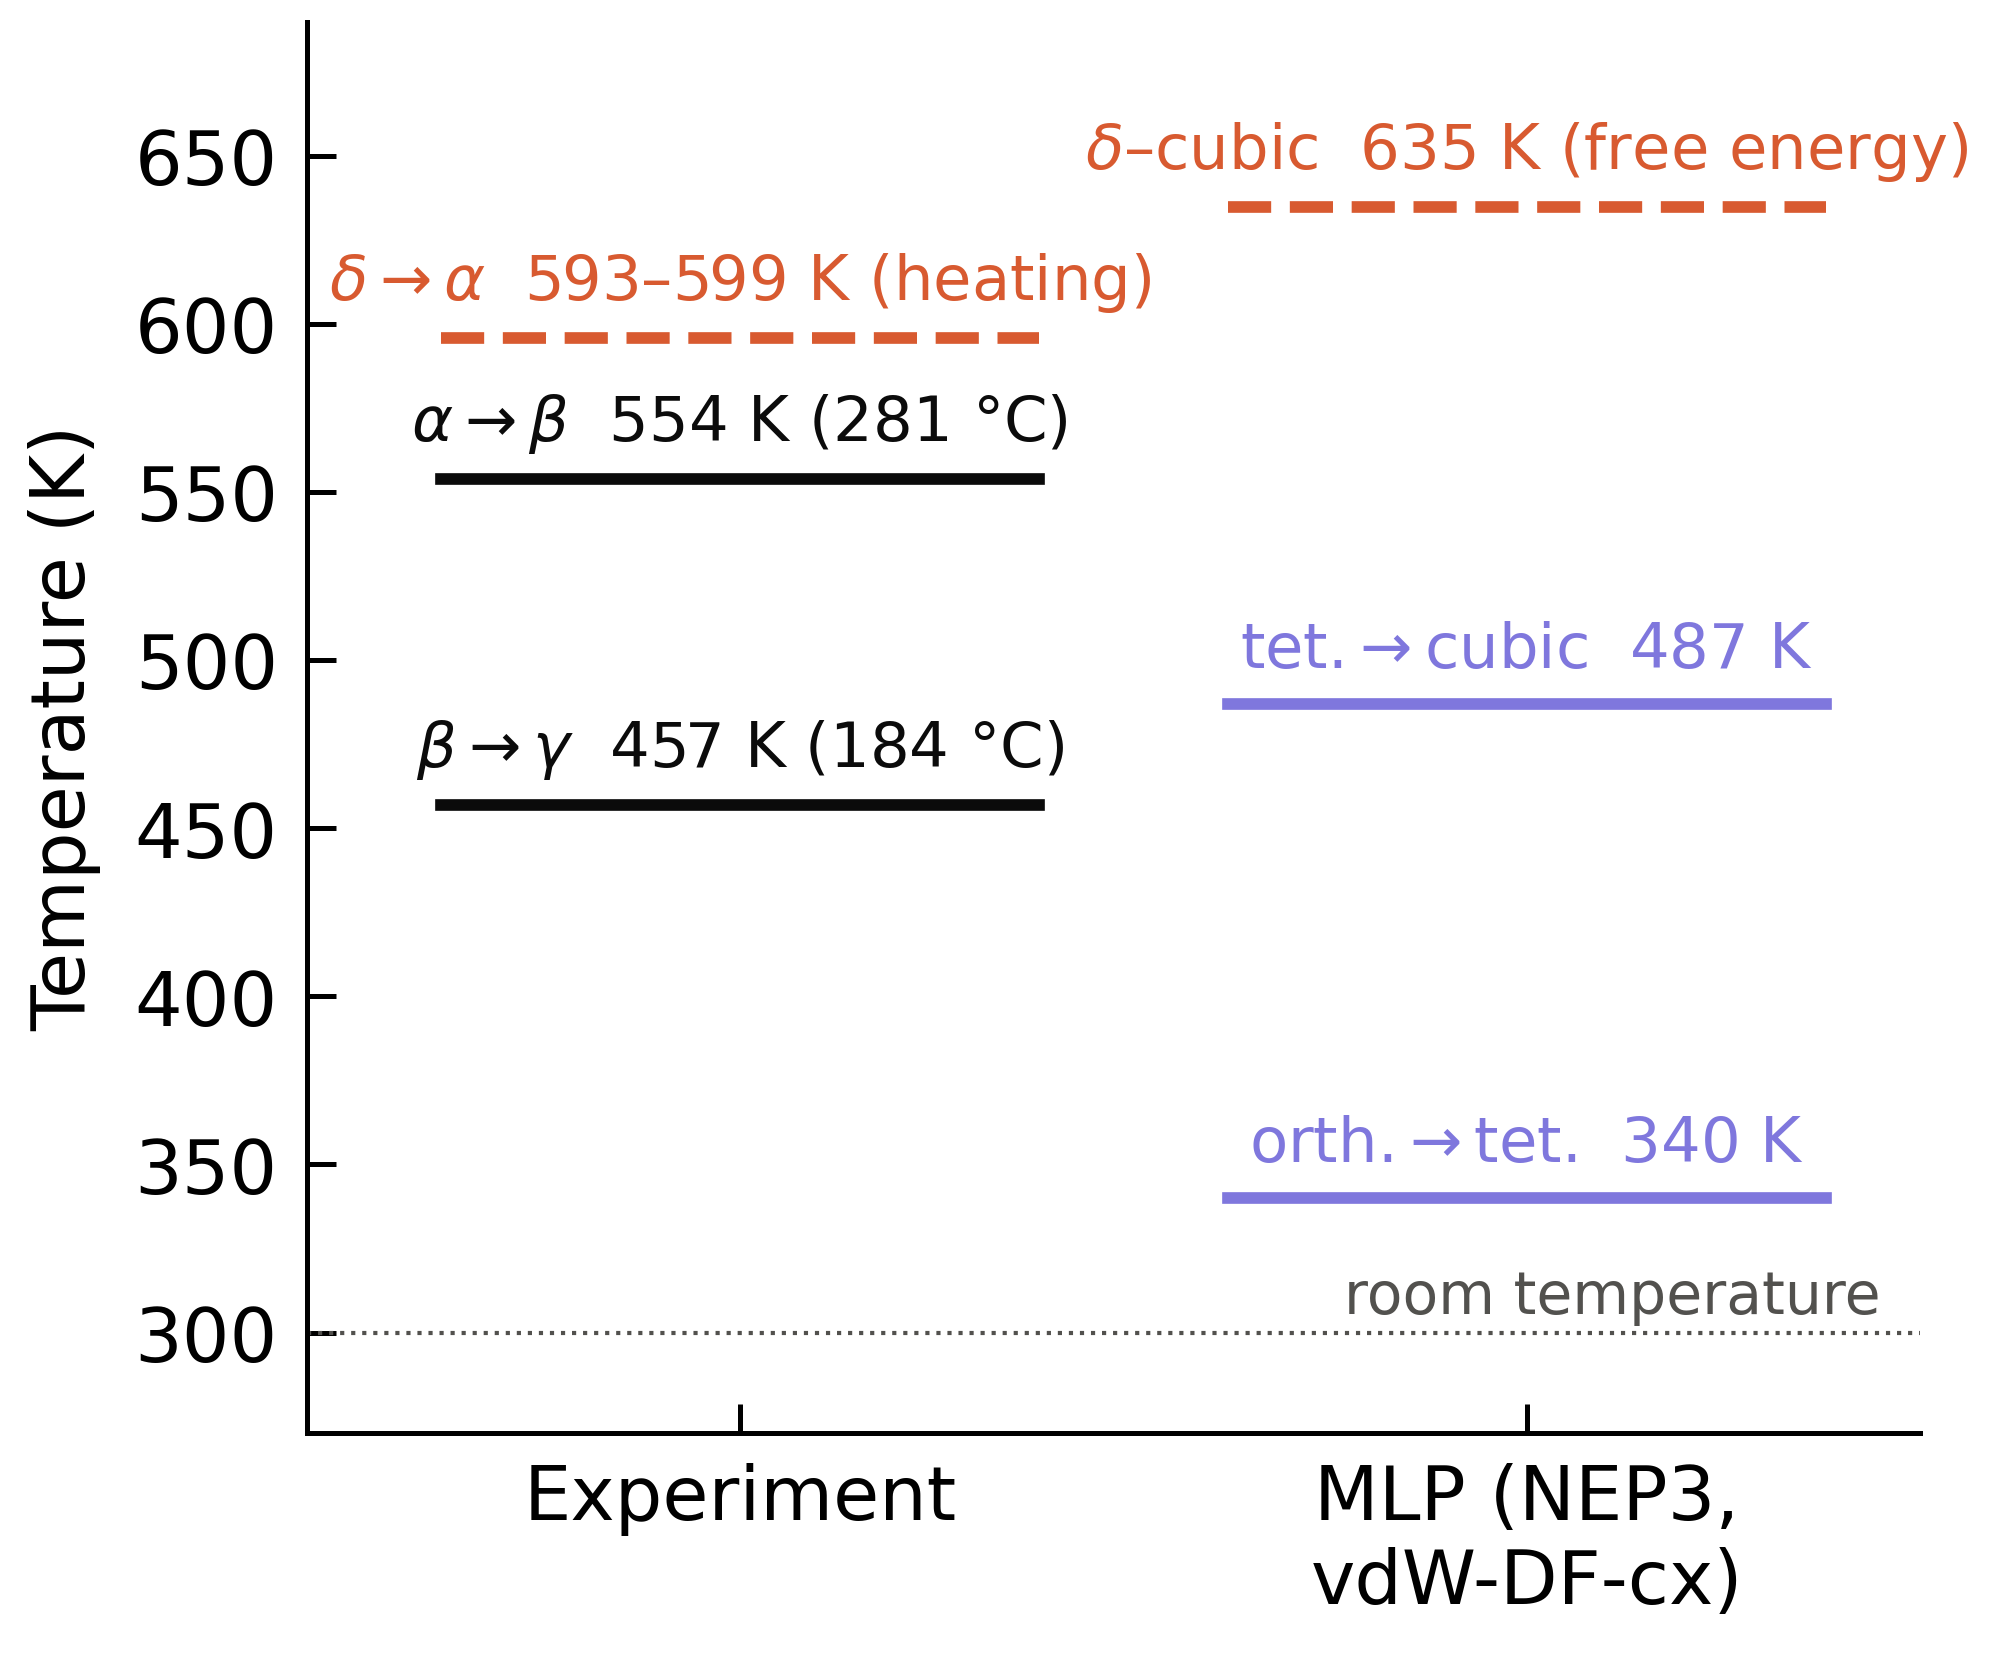
\includegraphics[width=\linewidth,height=0.74\textheight,keepaspectratio]{phase_ladder.png}
    \end{column}
    \begin{column}{0.5\textwidth}
      \small
      \begin{itemize}
        \item \textbf{Heating} $\delta$ turned black at 320--326\,$^\circ$C (593--599 K, DSC)\cit{3}.
        \item \textbf{Cooling} the black phase gave $\alpha\rightarrow\beta$ at 281\,$^\circ$C and $\beta\rightarrow\gamma$ at 184\,$^\circ$C (powder, 2.5\,$^\circ$C/min)\cit{1}.
        \item On cooling the crystal stays a perovskite, because $\delta$ cannot form fast. $\gamma$ survives at room temperature only for a while and then turns yellow\cit{3}.
        \item The equilibrium diagram is therefore simple ($\delta$ below about 600 K, $\alpha$ above), but the \textbf{kinetic} path decides what a film looks like.
      \end{itemize}
    \end{column}
  \end{columns}
  \refs{\RA\quad \RC}
\end{frame}

\begin{frame}{Experiment: thin films and strain}
  \small
  \begin{itemize}
    \item \textbf{Time--temperature--transformation map.} Holley \emph{et al.} followed films through heating, quenching and storage. The black phase at room temperature is a metastable state with a finite lifetime\cit{3}.
    \item \textbf{Substrate clamping.} Films quenched from 330\,$^\circ$C on glass or ITO kept about 1\,\% tensile strain and stayed black much longer than free-standing ones\cit{4}.
    \item \textbf{What sets the lifetime} besides strain: grain size and surface energy, humidity, and additives. None of these change the bulk ground state.
  \end{itemize}
  \begin{alertblock}{Reading}
    \small Experiment fixes the transition temperatures well. It cannot show the free-energy difference between $\gamma$ and $\delta$ at room temperature, which is where simulation comes in.
  \end{alertblock}
  \refs{\RC\quad \RD}
\end{frame}

\begin{frame}{How a machine-learned potential gets a phase diagram}
  \small
  \begin{enumerate}
    \item \textbf{Train} a potential (NEP3, MACE, \ldots) on DFT energies and forces of all phases, at several temperatures.
    \item \textbf{Displacive transitions} ($\alpha$, $\beta$, $\gamma$): heat and cool cells of tens of thousands of atoms in MD. The transition shows as a peak in the heat capacity and a jump in the octahedral tilt. Rates below about 30--60 K/ns and large cells are needed for converged values\cit{5}.
    \item \textbf{Reconstructive transition} ($\delta$): too slow for MD. Instead the free energy of each phase is computed (thermodynamic integration, Frenkel--Ladd), and the crossing gives the transition temperature\cit{5,6,7}.
  \end{enumerate}
  \vspace{0.3em}
  \textbf{Key point.} The potential only reproduces its training functional. The functional therefore decides the answer, not the machine learning\cit{5,6}.
  \refs{\RE\quad \RF\quad \RG}
\end{frame}

\begin{frame}{MLP results}
  \begin{columns}[c]
    \begin{column}{0.5\textwidth}
      \centering
      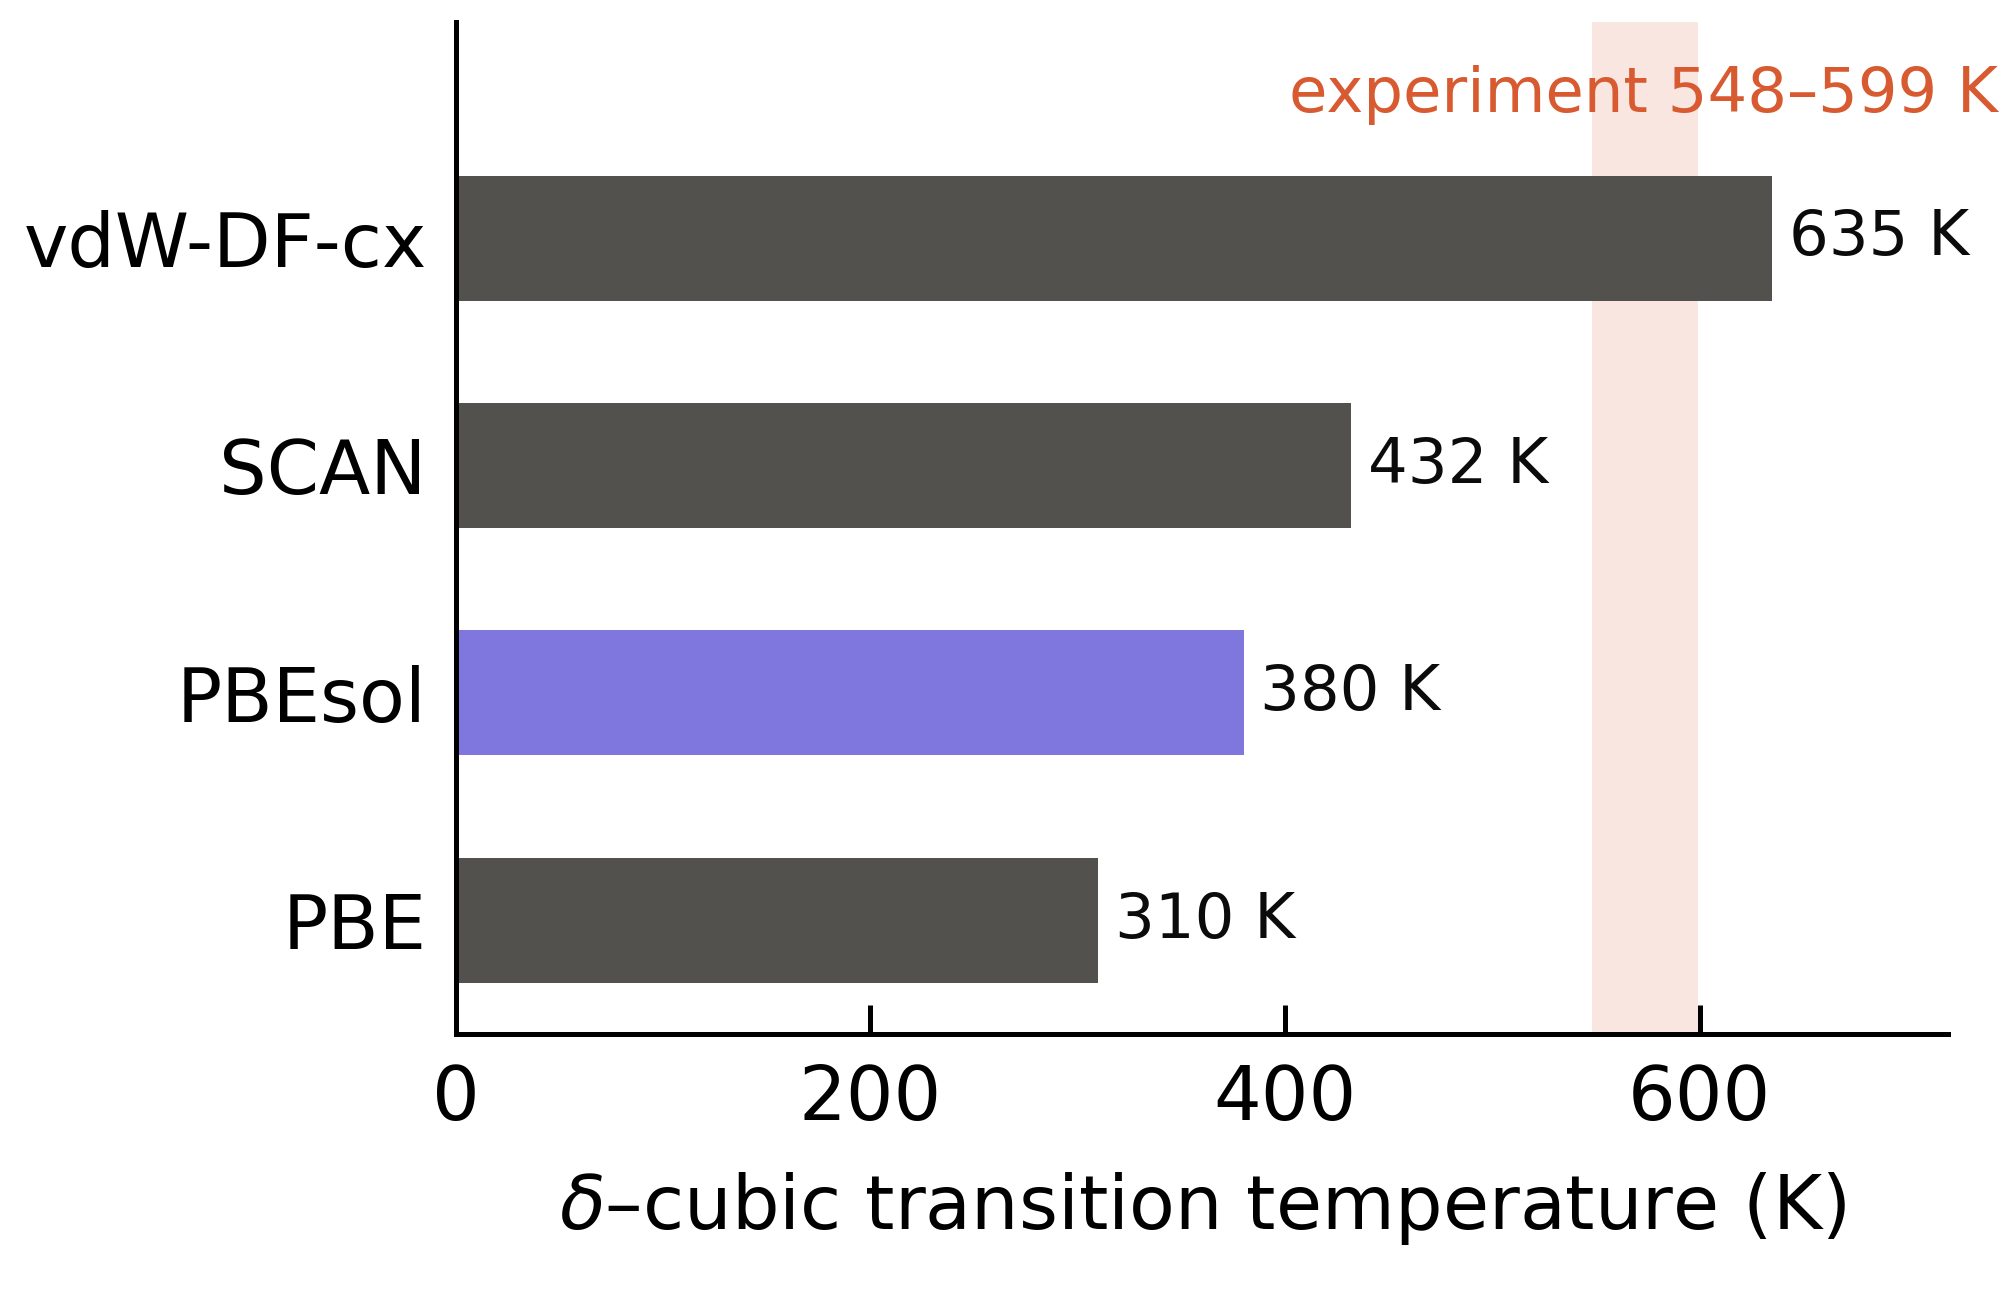
\includegraphics[width=\linewidth,height=0.62\textheight,keepaspectratio]{phase_delta_functional.png}
    \end{column}
    \begin{column}{0.48\textwidth}
      \scriptsize
      \begin{itemize}
        \item \textbf{Fransson \emph{et al.}}\cit{5}, NEP3 (GPUMD): orth.\,$\rightarrow$\,tet.\ 340 K and tet.\,$\rightarrow$\,cubic 487 K with vdW-DF-cx, the best of the tested functionals. Semi-local functionals underestimated these by up to 200 K.
        \item Same work, $\delta$--cubic by free energy: \textbf{635 K} (vdW-DF-cx), 432 K (SCAN), \textbf{380 K (PBEsol)}, 310 K (PBE), against about 600 K measured.
        \item \textbf{Braeckevelt \emph{et al.}}\cit{6}: RPA benchmark of the functionals. An unsuitable functional missed the transition by more than 100 K; the validated set reproduced experiment.
        \item \textbf{Braeckevelt \emph{et al.}}\cit{7}, MACE (PBE+D3): $\delta\rightarrow\gamma$ in line with the measured 548--599 K.
      \end{itemize}
    \end{column}
  \end{columns}
  \refs{\RE\quad \RF\quad \RG}
\end{frame}

\begin{frame}{What this means for the strain study}
  \small
  \begin{itemize}
    \item \textbf{PBEsol places the $\delta$--perovskite crossing at 380 K}, about 220 K below experiment\cit{5}. PBEsol therefore underestimates how much more stable $\delta$ is.
    \item The PBEsol gap of this work, $\Delta E_{\gamma\delta}$ = 79 meV per formula unit, is then likely a \textbf{lower bound} on the true gap.
    \item \textbf{Strain differences are safer} than the absolute gap: the change $\Delta E_{\gamma\delta}(\varepsilon) - \Delta E_{\gamma\delta}(0)$ depends far less on the functional.
    \item \textbf{Cheap check:} single points of the relaxed $\gamma$ and $\delta$ unit cells (20 atoms each) with vdW-DF-cx or SCAN give the size of the functional error for 79 meV.
  \end{itemize}
  \begin{alertblock}{Summary}
    \small $\delta$ is the ground state below about 600 K; the black phase at room temperature is kinetic. MLPs reproduce the sequence when trained on a suitable functional, and PBEsol underestimates the $\delta$ stability.
  \end{alertblock}
  \refs{\RE}
\end{frame}

\begin{frame}{References}
  \tiny
  \begin{itemize}\setlength{\itemsep}{1pt}
    \item[] \RA
    \item[] \RB
    \item[] \RC
    \item[] \RD
    \item[] \RE
    \item[] \RF
    \item[] \RG
  \end{itemize}
\end{frame}

\end{document}
